\documentclass{article}

% if you need to pass options to natbib, use, e.g.:
% \PassOptionsToPackage{numbers, compress}{natbib}
% before loading nips_2017
%
% to avoid loading the natbib package, add option nonatbib:
% \usepackage[nonatbib]{nips_2017}

\usepackage[final]{nips_2017}

% to compile a camera-ready version, add the [final] option, e.g.:
% \usepackage[final]{nips_2017}

\usepackage[utf8]{inputenc} % allow utf-8 input
\usepackage[T1]{fontenc}    % use 8-bit T1 fonts
\usepackage{hyperref}       % hyperlinks
\usepackage{url}            % simple URL typesetting
\usepackage{booktabs}       % professional-quality tables
\usepackage{amsfonts}       % blackboard math symbols
\usepackage{nicefrac}       % compact symbols for 1/2, etc.
\usepackage{microtype}      % microtypography
\usepackage{graphicx}

\title{CNN Assistance in Jigsaw Puzzle Solution}

% The \author macro works with any number of authors. There are two
% commands used to separate the names and addresses of multiple
% authors: \And and \AND.
%
% Using \And between authors leaves it to LaTeX to determine where to
% break the lines. Using \AND forces a line break at that point. So,
% if LaTeX puts 3 of 4 authors names on the first line, and the last
% on the second line, try using \AND instead of \And before the third
% author name.

\author{Tianbao Li\\
  Department of Computer Science\\
  University of Toronto\\
  Toronto, ON M5S 1A1 \\
  \texttt{tianbao@cs.toronto.edu} \\
  %% examples of more authors
  %% \And
  %% Coauthor \\
  %% Affiliation \\
  %% Address \\
  %% \texttt{email} \\
  %% \AND
  %% Coauthor \\
  %% Affiliation \\
  %% Address \\
  %% \texttt{email} \\
  %% \And
  %% Coauthor \\
  %% Affiliation \\
  %% Address \\
  %% \texttt{email} \\
  %% \And
  %% Coauthor \\
  %% Affiliation \\
  %% Address \\
  %% \texttt{email} \\
}

\begin{document}
% \nipsfinalcopy is no longer used

\maketitle

\begin{abstract}

This paper presents an innovative way to assist solving jigsaw puzzle with the help of deep convolutional neural networks. The main goal of this project is to predict whether two pieces from the jigsaw puzzle should be neighbors in the origin image. Proceeding from traditional methods of using color (like RGB) distance, here, we introduce the low level features in the image which are extracted by convolutional neural networks. Compared with color-based solutions, using the feature maps generated can help with a deeper intuition on the correlation between edges. The proposed algorithm can achieve considerable accuracy on adjacency prediction.

\end{abstract}

\section{Introduction}

Jigsaw puzzles were first introduced around 1760 for map research and then became a popular intelligence entertainment \cite{freeman1964apictorial} in the last few centuries. The origin image is divided into $N\times M$. To solve this, people need to cluster similar tiles, find the neighbors and then reconstruct the origin image. However, due to the possible locations and relationship behind pieces, there are quite a huge number of solutions ever for a small jigsaw puzzle, for example, $(8*8)!=1.2688693*10^{89}$ solutions for an $8*8$ puzzle. Indeed, this problem has be proven to be a NP-complete one \cite{altman1989solving,demaine2007jigsaw}. Though tough, actually, jigsaw puzzle solving is quite meaningful beyond the intelligence challenge. It helps a lot in combining shredded of documents \cite{levin1975computer,marques2009reconstructing} and even recovering artifacts debris\cite{koller2006computer}.

Recently year, there have been a lot researchers working on this problem and achieved much progress. However, one the the most important sub-problems in this procedure, determining adjacency between pieces, seems keeps in the same track for long. When people solve the puzzle manually, they need needs image information at edges, such as color, texture, instance, etc. to make the judgment whether two pieces are neighbors. However, most of previous research only eyes on the color features such as RGB distance. This make such solutions quite bad for simple-colored images, especially in reconstructing printed documents of ancient artifacts.

Here, we want to mimic how people really solve jigsaw puzzles and work on finding features capable to help make adjacent prediction. Recently, Convolution Neural Networks (CNN) leads the research area of computer vision with its capability of extracting inside features underneath the images and sole hard problems such as detection\cite{redmon2017yolo9000} and segmentation\cite{he2017mask,yu2015multi}. Based on the existing tremendous structures, people start to apply transfer learning and use extracted features to solve related computer vision problems\cite{razavian2014cnn}.

In this paper, we contribute in providing neural networks to predict whether two tiles from a jigsaw puzzle are adjacent in the origin image. The neural networks judge the jigsaw piece pair by extracted low lever image features from pre-trained CNN together with color information at edges, and outputs whether this two tiles are neighbors. This model achieves outstanding prediction accuracy in images from ILSVRC2012 dataset\cite{ILSVRC15}.

\section{Related Work}

Jigsaw has been researched on for many years. One most basic idea is to evaluate the compatibility of the adjacent pieces and take a strategy, such as greedy search, to arrange the pieces. One famous work is the Genetic Algorithm (GA) \cite{sholomon2013genetic}. Given initial candidate solutions, it applies operations like selection, reproduction and mutation based on the color-distance fitness function. Similarly but innovative, \cite{sholomon2016dnn} first introduces deep neural network to jigsaw solver and transforms the puzzle to the piece pair adjacency prediction. It samples piece edges to learn the adjacent likelihood through DNN based on the color distance. For these two solvers, they only use color information to judge whether two pieces should be together. However, human use some others like texture to solve. Also, though high accuracy, these solution could not solve the jigsaw puzzle which generated by single-colored or colorless images. So, there are still some further steps on it.

Recently, with the prosper of convolutional neural networks in computer vision area, convolutional neural networks (CNN) also becomes a good tool to solve jigsaw puzzles. Because of the fact that a good CNN is hard to train and the training data needs many images and well labels, more and more researchers choose the apply transfer learning on pre-trained models, fine turning on the last a few layers or using it as a feature extractor, instead of go over all the process \cite{razavian2014cnn}. CNN can extract regional features in many perspectives, such as color, texture, pattern, instance. Features in the formers usually reflect the basic information of the images, while the latter layers can make high-level judgement. These can be good inference for judging adjacent pieces. So, \cite{deryneural,noroozi2016unsupervised} choose to use feature maps from pre-trained CFN \cite{noroozi2016unsupervised} (siamese-ennead AlexNet \cite{krizhevsky2012imagenet}), VGG \cite{he2016deep} or Resnet \cite{simonyan2014very} and predict the location. However, the main problem for these approach is that they hold a siamese structure with shared weights for each location, which means they can only solve a limited number for pieces ($3\times3$ in \cite{noroozi2016unsupervised}, $2\times2$ and $2\times3$ in \cite{deryneural}). With the piece amount increasing, the network becomes extremely heavy to train.

\section{Preliminary}

\subsection{Problem Definition}

Jigsaw puzzles aims to reshape multiple non-overlapping pieces from the origin image to the correct arrangement. In our project, like in most computer research, we focus on equal-sized squared $W=N\times M$ pieces. It refuses the aid of shape matching but asks for more on image information. The expected result is a set of indexes $I=(p_1,p_2,\dots,p_W)$ which $p_i$ is the corresponding index for each piece in the origin image. For the worst case, it takes the complicity of $O(W!)$. For example, Figure~\ref{fig:colorfuljigsawpuzzle} is a $3*3$ jigsaw puzzle. The left subgraph is the origin image, and the right subgraph is the puzzle which $I=\{6,2,7,3,5,4,0,8,1\}$.

\begin{figure}
    \begin{minipage}{\textwidth}
        \begin{minipage}{.49\textwidth}
            \begin{minipage}{.49\textwidth}
                \centering
                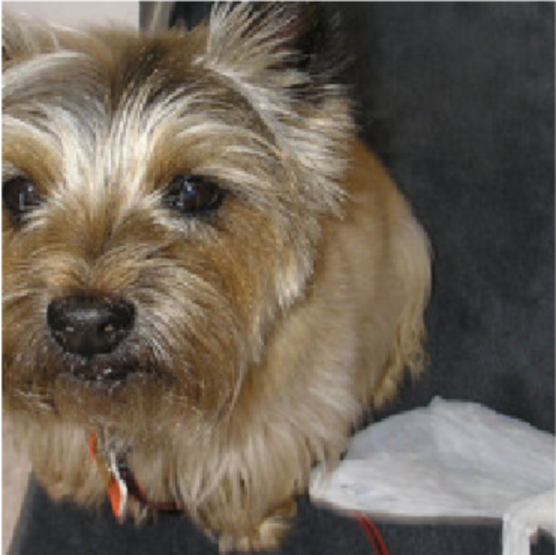
\includegraphics[width=\textwidth]{origin_color}
            \end{minipage}
            \begin{minipage}{.49\textwidth}
                \centering
                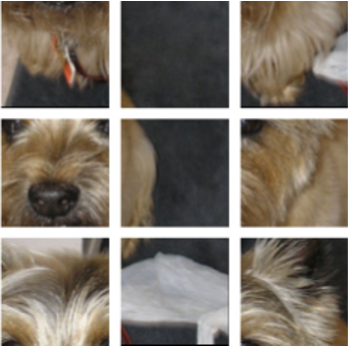
\includegraphics[width=\textwidth]{puzzle_color}
            \end{minipage}
            \caption{Colorful Jigsaw Puzzle Example}
            \label{fig:colorfuljigsawpuzzle}
        \end{minipage}
        \begin{minipage}{.49\textwidth}
            \begin{minipage}{.49\textwidth}
                \centering
                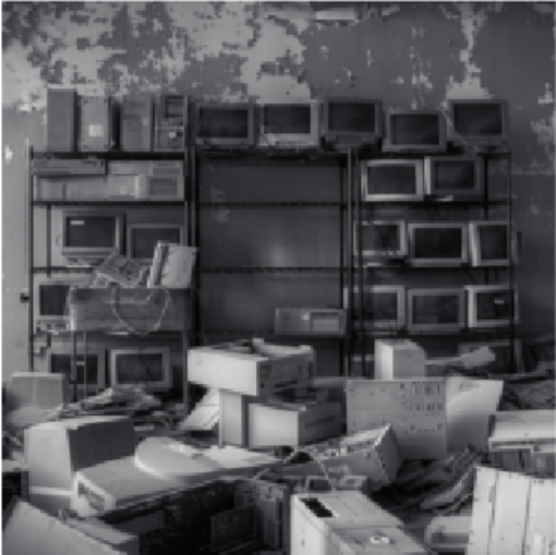
\includegraphics[width=\textwidth]{origin_black}
            \end{minipage}
            \begin{minipage}{.49\textwidth}
                \centering
                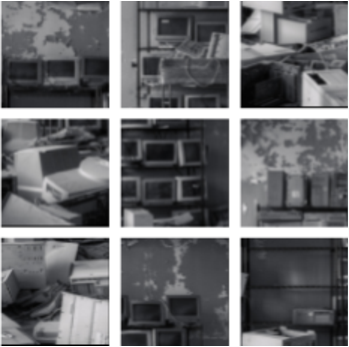
\includegraphics[width=\textwidth]{puzzle_black}
            \end{minipage}
            \caption{Black Jigsaw Puzzle Example}
            \label{fig:blackjigsawpuzzle}
        \end{minipage}
    \end{minipage}
    \begin{minipage}{\textwidth}
        \begin{minipage}{.49\textwidth}
            \begin{minipage}{.49\textwidth}
                \centering
                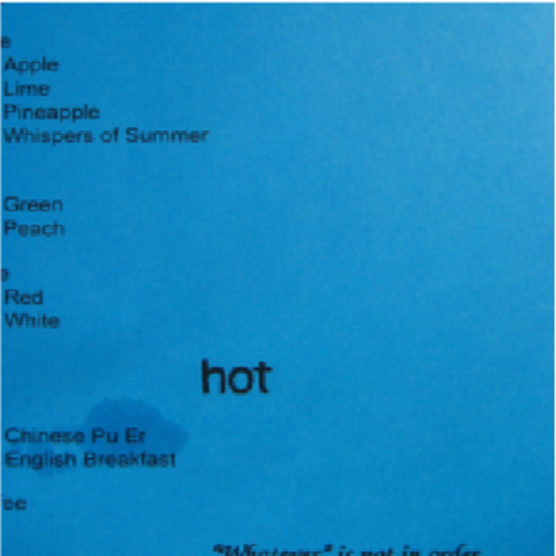
\includegraphics[width=\textwidth]{origin_blue}
            \end{minipage}
            \begin{minipage}{.49\textwidth}
                \centering
                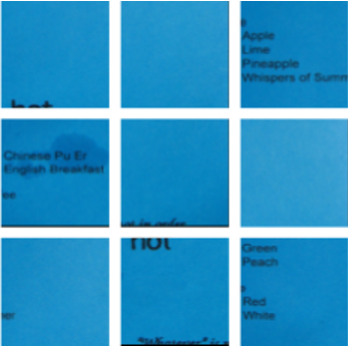
\includegraphics[width=\textwidth]{puzzle_blue}
            \end{minipage}
            \caption{Blue Jigsaw Puzzle Example}
            \label{fig:bluejigsawpuzzle}
        \end{minipage}
        \begin{minipage}{.49\textwidth}
            \begin{minipage}{.49\textwidth}
                \centering
                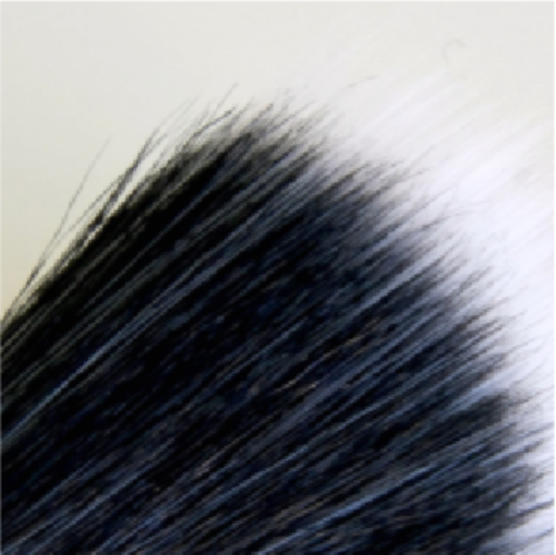
\includegraphics[width=\textwidth]{origin_texure}
            \end{minipage}
            \begin{minipage}{.49\textwidth}
                \centering
                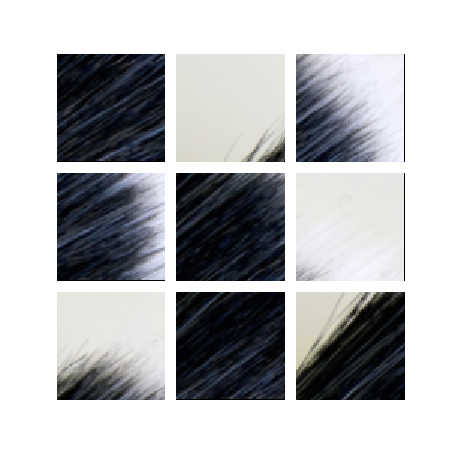
\includegraphics[width=\textwidth]{puzzle_texure}
            \end{minipage}
            \caption{Textural Jigsaw Puzzle Example}
            \label{fig:texurejigsawpuzzle}
        \end{minipage}
    \end{minipage}
\end{figure}

\subsection{Motivation}

Starting from the idea in \cite{sholomon2016dnn}, instead of solving the jigsaw puzzle from the from to the end, we choose to focus on the prediction whether two jigsaw puzzle tile should be neighbor in the origin image. In recent research, nearly all of the researchers decide to use color information to judge whether two tiles are adjacent. And as in the result, the color distance like RGB distance appears as a good measurement. In some work\cite{sholomon2013genetic} the color distance is defined as the sum of squared color differences in three-dimensional color space like RGB. For image piece $x_i$ and $x_j$ as a $K\times K\times 3$ matrix which $K$ is the edge length and $cb$ is the color band, the distance is
$$
D(x_i,x_j,r)=\sqrt[]{\sum^K_{k=1}\sum^3_{cb=1}(x_i(k,K,cb)-x_j(k,1,cb))^2}
$$

However, this color-based measurement doesn't work all the time. For example, in Figure~\ref{fig:blackjigsawpuzzle}, RGB-based can not predict the similarity of grey-scaled images. Also even changed it to grey-level distance, it doesn't work so well. Also, like in Figure~\ref{fig:bluejigsawpuzzle}, even in RGB band, main part of the image is in color blue, even all blue pixels in some edges. So the distances are so close for all edge pairs, which can leads to high error rate for the prediction. Moreover, for the images of furs, hairs and others with obvious pattern structure, like in Figure~\ref{fig:texurejigsawpuzzle}, it is easy to have a low distance with the displacement fitting the pattern though it is wrong. Only color information can not have a good result on this.

Here, we combine the features extracted from Resnet34\cite{he2016deep}. Usually, people choose the extract the feature maps after the activation functions which contains much image information such as color, texture and so on. Resnet34 is constructed on the structure of BasicBlock (several layers of convolutions, batch normalization, ReLUs, etc) and can skip some of the blocks to achieve the residual learning with more blocks. Resnet34 has 3, 4, 6 and 3 blocks in each section. There are some discussions in \cite{noroozi2016unsupervised} that feature maps from low layers of CNN can help with solving the jigsaw puzzle better. In our algorithm, we choose to use the ReLU output after the first block.

Combining the measurements above, the goal of the algorithm is to build the neural networks based classifier to predict the adjacent likelihood of a pair of two jigsaw puzzle edges in the origin image. Note that not all pixels help with the prediction near the edge, we only use the feature maps and color value for the two rows near the edge to reduce the work load of the neural networks.

\section{Adjacency Prediction Algorithms}

\subsection{BuddyNet}

In this section, we will discuss the neural network structure, BuddyNet. It is a NN classifier which predicts the adjacency likelihood of a pair of jigsaw tiles in the origin image.

As mentioned in the motivation, we want to extract low level features in Resnet34\cite{he2016deep}. Resnet34 has the structure of a combination of basic blocks as in Figure~\ref{fig:basicblock}. To extract features for each piece, we first resize it into the shape of $224\times 224$, which is the expected input size of Resnet34. After one convolotional layer of $7\times7$, the data is passed through the first basic block and output 64 feature maps which has the size of $56\times 56$. One example is shown as in Figure~\ref{fig:featuremapexample}. 64 small images on the right side are the feature maps of the piece on the left. We can see that some feature maps focus on different regions (the from object or the background), together with some others with more concentration on the shape and other content. To build the connection near the edges, we extract the two rows of pixels near the edge. In this way, we have $2\times 56\times 64=7168$ values to express the edge.

\begin{figure}
    \centering
    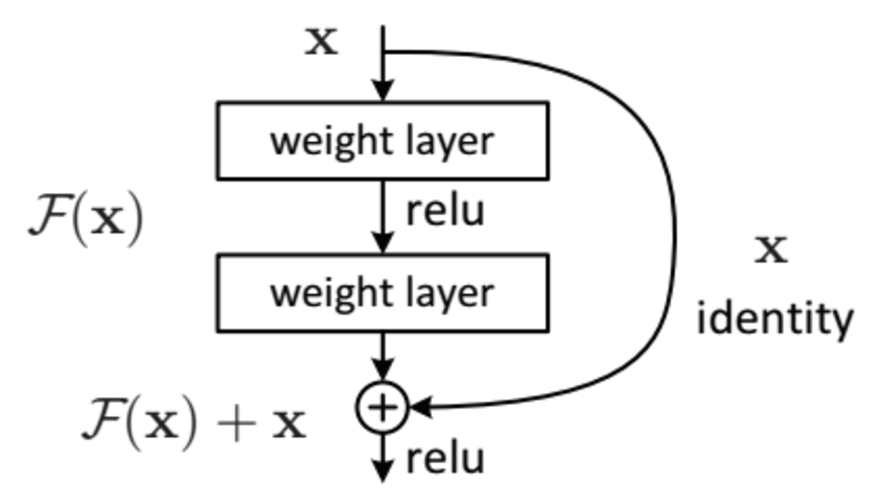
\includegraphics[width=0.5\textwidth]{basicblock}
    \caption{Basic Block of Resnet34}
    \label{fig:basicblock}
\end{figure}

\begin{figure}
    \centering
    \begin{minipage}{.30\textwidth}
        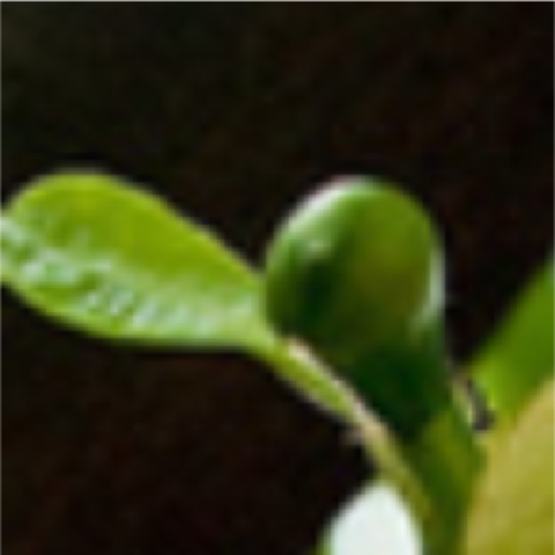
\includegraphics[width=\textwidth]{fmp_origin}
    \end{minipage}
    \hfill
    \begin{minipage}{.65\textwidth}
        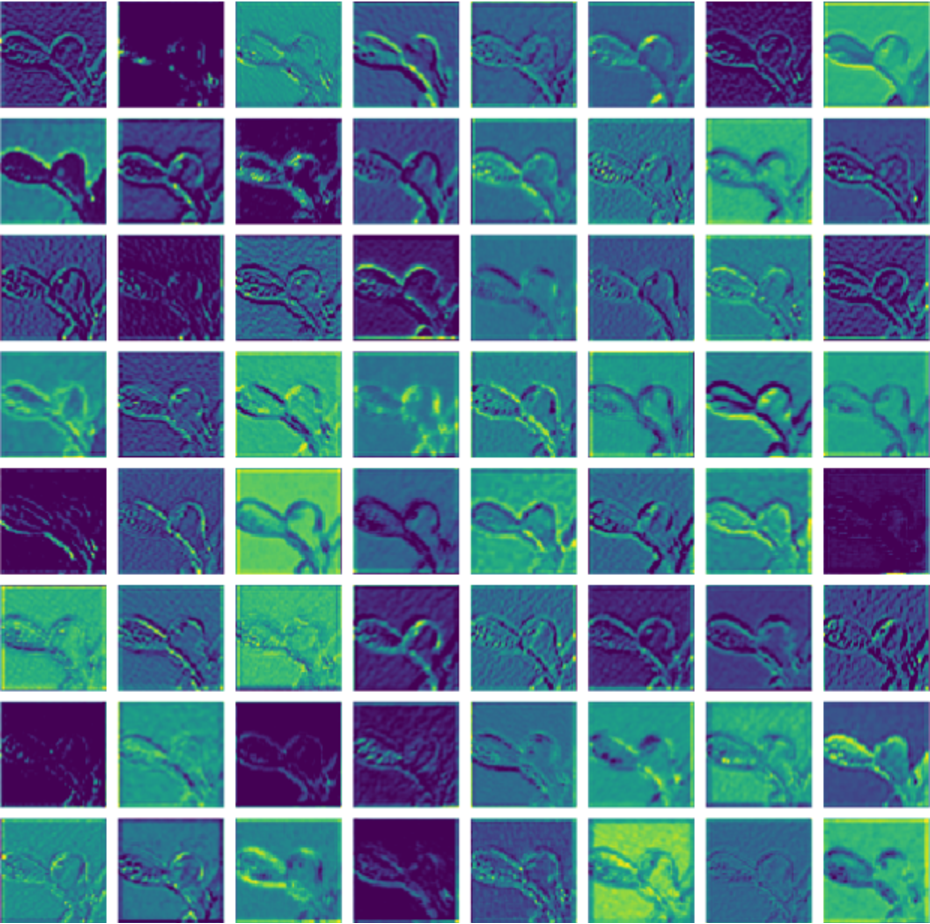
\includegraphics[width=\textwidth]{fmp}
    \end{minipage}
    \caption{Feature Map Example}
    \label{fig:featuremapexample}
\end{figure}

Also, as an import indicator of the image, we integrate the above features with RGB valve. With each pixel in the piece image has 3 color band, we have $2\times 224\times 3=1344$ values (2 rows with edge of 224 pixels).

To predict the adjacent likelihood, we integrate the information above and build a forward neural network. For a pair of piece edges, we transform the information into a vector with the size of $2*(7168+1344)=17024$ as the input. The network has 8 fully connected layers of size 8512, 8512, 2464, 2464, 672, 672, and 2. The output is a layer of 2 nodes generated by ReLU activation function. The expected output is (1,0) for neighbor pair (positive) and (0,1) for non-neighbor pair (negative). All the activation is the network is ReLU. The structure of the network is shown as Figure~\ref{fig:buddynet}, with neurons amount at the bottom.

\begin{figure}
    \centering
    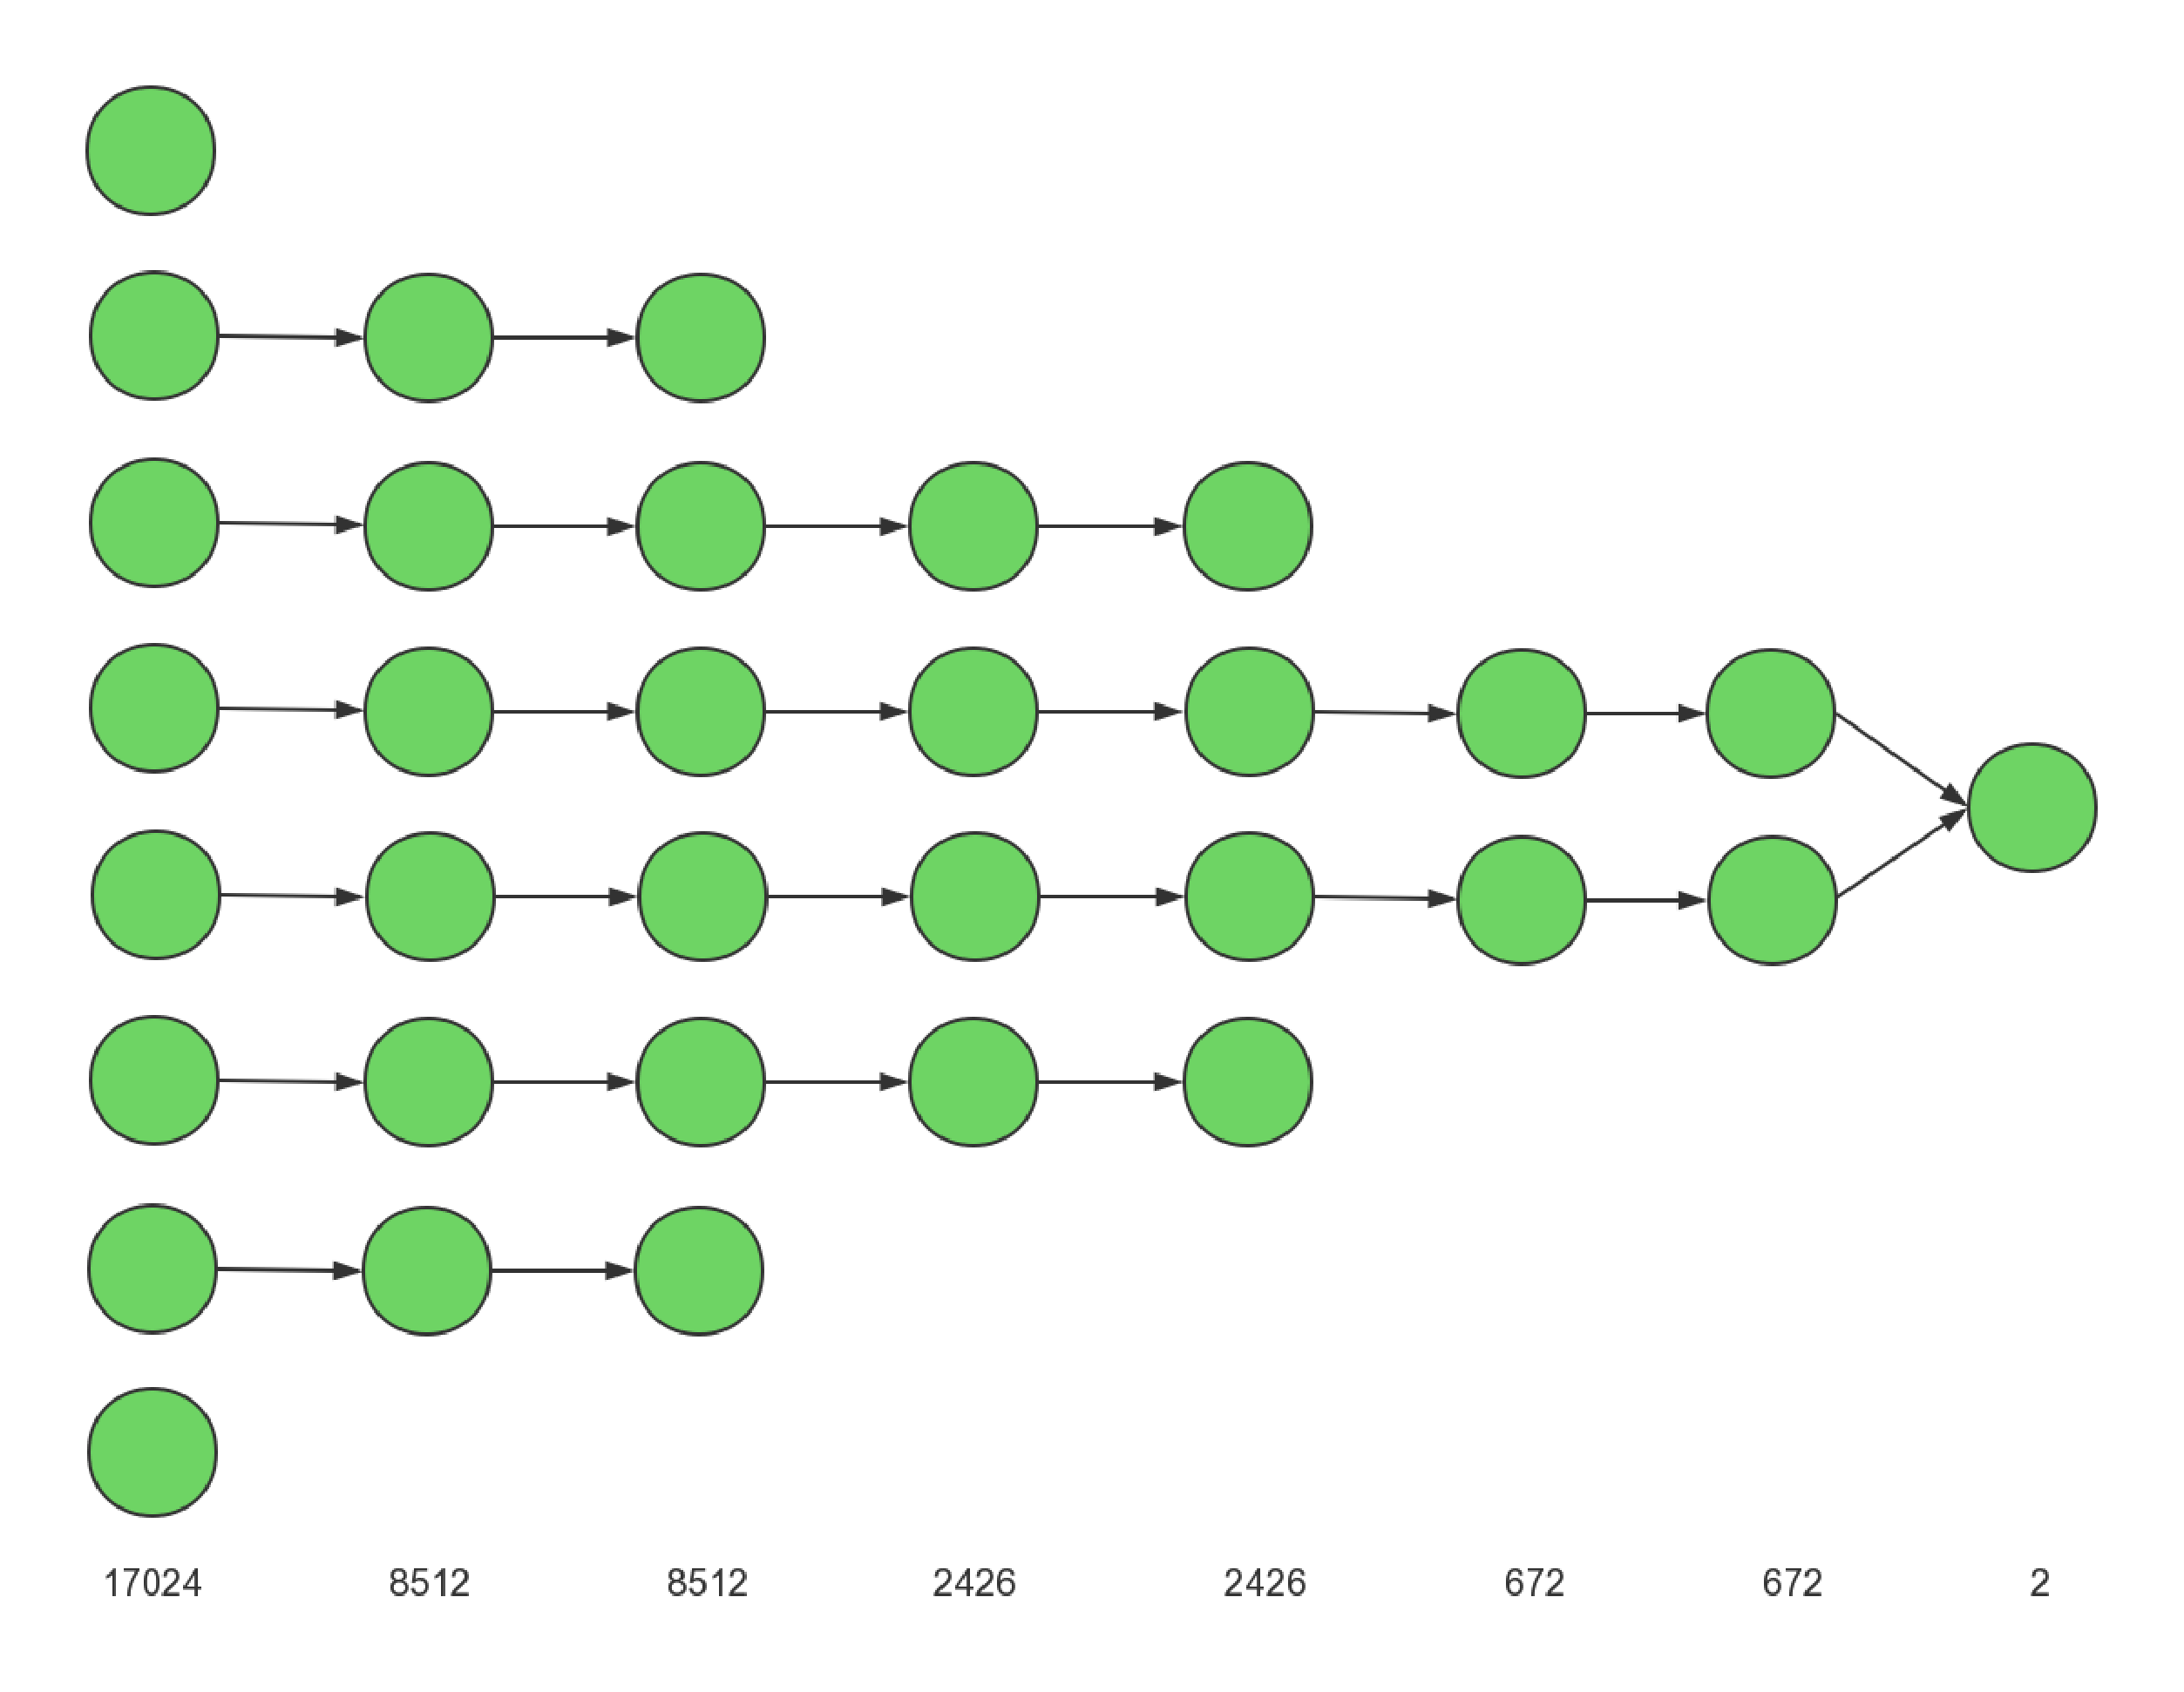
\includegraphics[width=0.8\textwidth]{BuddyNet}
    \caption{Architecture of BuddyNet}
    \label{fig:buddynet}
\end{figure}

Additionly, to test how our proposed neural network works for grey-scaled images, we change the architecture into a new version without integrating RGB information. This network takes a vector with size of $2*7168=14336$ as the input, and hidden layers have 7168, 7168, 1792, 1792, 448, 448, and 2 neurons. Other parameters are just the same as previous BuddyNet.

\subsection{RGBNet}

As used in many popular solutions, RGB distance has fairly good result in neighbor piece prediction. Here, to test the capability of expressing the image, we also build a forward neural network only using RGB value. The structure is similar to the one in \cite{sholomon2016dnn}, but we make some revision to achieve a higher accuracy. This RGBNet has 6 fully conencted layers, which the amounts of neurons are 2688, 1344, 672, 168, 42, and 2.

\section{Evaluation}

\subsection{Pre-trained Model and Dataset}

Instead of training Resnet34 for a huge amount of time, here we choose to use the pre-trained in the version of PyTorch\footnote{\url{https://download.pytorch.org/models/resnet34-333f7ec4.pth}}. Other neural networks are also implemented by PyTorch\footnote{\url{https://www.pytorch.org/}}. The Resnet34 models above is pre-trained on ImageNet\cite{krizhevsky2012imagenet} to learn the general expression of images.. To make the evaluation result more persuable, we seperate ImageNet validation set into training and validation set for this project.

The ImageNet validation set has 51003 images in total. The image sizes differ, so we apply random crop on this to $224\times224$. Next, each image is divided into tiles. In this evaluation, we try on $3\times3$ with edge length of 75 pixels and $8\times8$ with edge length of 28 pixels. Then we pass pieces through Resnet34, get the feature maps and generate the vector mentioned above together with RGB bands.

\subsection{Data Sampling}

For a jigsaw puzzle with $N$ pieces each edge, there are $N*N$ pieces in total and $(N*N)!$ possible combinations of piece pairs. However, only $2*N*(N-1)$ among them hold the positive label (actually adjacent in the origin image). Note that we do not consider rotated pieces by now. For the algorithm traing a classifier, it is extremely important to sample randomly and uniformly. If using the data above, classifying by giving prediction of ``false'' can get a high accuracy but low recall, not the classifier we want. To reduce the infuence caused by data inclining, we only sample $2*N*(N-1)$ pairs from the negative-labelled set (not adjacent ones) to keep a balanced dataset whose size is $4*N*(N-1)$.

In the end, we obtain balanced datasets of 100000 pairs for $3\times 3$ puzzle and 10000 pairs for  $8\times 8$ puzzle. We train the forward neural networks with Stochastic Gradient Descent to minimize the cross-entropy loss for 200 iterations and apply dropout (ratio = 0.5) for BuddyNet.

\subsection{Experiment Results}

In this section, we will give out the experiment result on changing different parameters, and analyze how the algorithms work and why is like that.

\textbf{algorithm}

The comparision on different algorithms are shown in Table~\ref{tab:expalg}. From the table we can see that the algorithms based on by bands only surpasses out proposed BuddyNet with a margin. And out revised one has a little higher accuracy than DNN\_Buddies\cite{sholomon2016dnn}.

Actually, there are only 4916 neurons in the archetichure but 23298 in the proposed BuddyNet. The structure is much more complicated than those and requires more training data to overcome underfitting. Also, we can see that there is stilla largin margin between training accuracy and validation accuracy for BuddyNet, more data can help.

\begin{table}
    \caption{Experiement Results on Different Algorithms}
    \centering
    \label{tab:expalg}
    \begin{tabular}{c|c|c|c|c}
        \hline
        & data amount & pieces & training accuracy & validation accuracy\\
        \hline
        BuddyNet & 10000 & $3\times 3$ & 0.9546 & 0.9395\\
        \hline
        RGBNet & 10000 & $3\times 3$ & 0.9904 & 0.9861\\
        \hline
        \hline
        DNN-Buddies \cite{sholomon2016dnn} & 10000 & $3\times 3$ & 0.9858 & 0.9846\\
        \hline
    \end{tabular}
\end{table}

\textbf{data amount}

The comparision on different training data sizes are shown in Table~\ref{tab:expamount}. From the table we can see that more training data help the models achieve a better result on accuracy, especially for BuddyNet with a complicated structure as discussed above. Also, the existing margin between training accuracy and validation shows there is still potential for BuddyNet.

\begin{table}
    \caption{Experiement Results on Different Training Data Sizes}
    \centering
    \label{tab:expamount}
    \begin{tabular}{c|c|c|c|c}
        \hline
        & data amount & pieces & training accuracy & validation accuracy\\
        \hline
        BuddyNet & 10000 & $3\times 3$ & 0.9546 & 0.9395\\
        \hline
        BuddyNet & 100000 & $3\times 3$ & 0.9912 & 0.9749\\
        \hline
        RGBNet & 10000 & $3\times 3$ & 0.9904 & 0.9861\\
        \hline
        RGBNet & 100000 & $3\times 3$ & 0.9976 & 0.9947\\
        \hline
    \end{tabular}
\end{table}

\textbf{pieces}

The comparision on different piece amounts on each edge are shown in Table~\ref{tab:exppiece}. From the table we can see that prediction on $3\times 3$ pieces (edge length of 75) is better than $8\times 8$ (edge length of 28) from the same size of the origin image. This is easy to understand because the feature maps and RGB bands we use are all in the pixel level. Fewer pixels means less information we have, leading to worse prediction. So, for the low resolution pieces, applying super resolution methods before passing through Resnet34 may help work better.

\begin{table}
    \caption{Experiement Results on Different piece amounts}
    \centering
    \label{tab:exppiece}
    \begin{tabular}{c|c|c|c|c}
        \hline
        & data amount & pieces & training accuracy & validation accuracy\\
        \hline
        BuddyNet & 10000 & $3\times 3$ & 0.9546 & 0.9395\\
        \hline
        RGBNet & 10000 & $3\times 3$ & 0.9904 & 0.9861\\
        \hline
        BuddyNet & 10000 & $8\times 8$ & 0.9277 & 0.8945\\
        \hline
        RGBNet & 10000 & $8\times 8$ & 0.9488 & 0.9301\\
        \hline
    \end{tabular}
\end{table}

\textbf{color}

The result of grey-scaled BuddyNet are shown in Table~\ref{tab:expgrey}. We the use BuddyNet which only accepts feature maps as from Resnet34. From the table we can see that the accuracy is fairly good since grey-scaled jigswa puzzle is impossible for RGB-based solutions.

\begin{table}
    \caption{Experiement Results on Grey-scaled Images}
    \centering
    \label{tab:expgrey}
    \begin{tabular}{c|c|c|c|c}
        \hline
        & data amount & pieces & training accuracy & validation accuracy\\
        \hline
        BuddyNet\_grey & 10000 & $3\times 3$ & 0.8142 & 0.7693\\
        \hline
        BuddyNet\_grey & 100000 & $3\times 3$ & 0.8430 & 0.8085\\
        \hline
    \end{tabular}
\end{table}


\bibliographystyle{plain}
\bibliography{Jigsaw-Puzzle-Solver}

\end{document}
